\begin{figure}[H]
    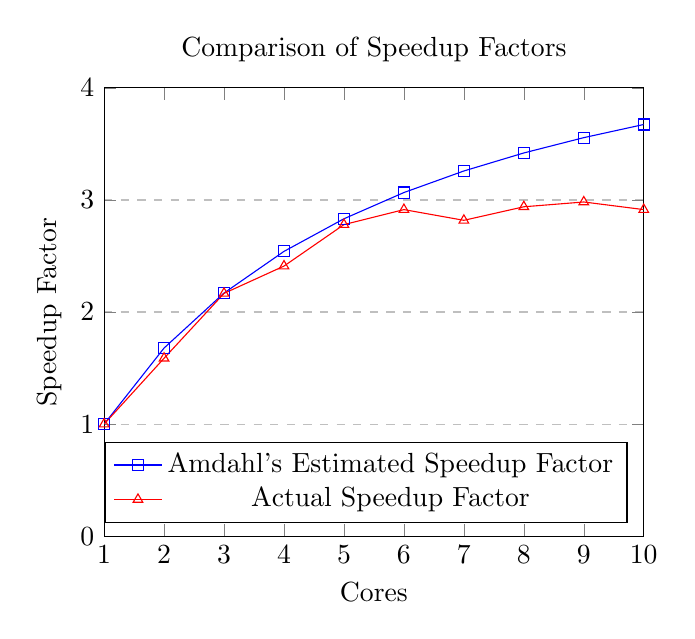
\begin{tikzpicture}
    \begin{axis}[
        title={Comparison of Speedup Factors},
        xlabel={Cores},
        ylabel={Speedup Factor},
        xmin=1, xmax=10,
        ymin=0, ymax=4,
        xtick={1,2,3,4,5,6,7,8,9,10},
        ytick={0,1,2,3,4},
        legend pos=south east,
        ymajorgrids=true,
        grid style=dashed,
    ]
    
    \addplot[
        color=blue,
        mark=square,
        ]
        coordinates {
        (1,1)(2,1.6787346222)(3,2.1695941855)(4,2.5411013569)(5,2.8320683114)(6,3.0661245456)(7,3.2584795325)(8,3.4193663866)(9,3.5559232301)(10,3.6732810342)
        };
        \addlegendentry{Amdahl's Estimated Speedup Factor}
    
    \addplot[
        color=red,
        mark=triangle,
        ]
        coordinates {
        (1,1)(2,1.5877659574)(3,2.1663138796)(4,2.4100925147)(5,2.7799767171)(6,2.9139719341)(7,2.8182533438)(8,2.9390769231)(9,2.9818938606)(10,2.9139719341)
        };
        \addlegendentry{Actual Speedup Factor}
    
    \end{axis}
    \end{tikzpicture}
    \caption{A comparison on the estimated speedup factor from Amdahl's law and the actual Speedup factor for 3DM on DUT 2}\label{fig:amdahls}
\end{figure}
